%%%%%%%%%%%%%%%%%%%%%%%%%%%%%%%%%%%%%%%%%%%%%%%%%%%%%%%%%%%%%%%%%%%%%%%%%%%%%%%%
%
% Template license:
% CC BY-NC-SA 3.0 (http://creativecommons.org/licenses/by-nc-sa/3.0/)
%
%%%%%%%%%%%%%%%%%%%%%%%%%%%%%%%%%%%%%%%%%%%%%%%%%%%%%%%%%%%%%%%%%%%%%%%%%%%%%%%%

%----------------------------------------------------------------------------------------
%	PACKAGES AND OTHER DOCUMENT CONFIGURATIONS
%----------------------------------------------------------------------------------------

\documentclass[
11pt, % The default document font size, options: 10pt, 11pt, 12pt
%oneside, % Two side (alternating margins) for binding by default, uncomment to switch to one side
%chapterinoneline,% Have the chapter title next to the number in one single line
spanish,
singlespacing, % Single line spacing, alternatives: onehalfspacing or doublespacing
%draft, % Uncomment to enable draft mode (no pictures, no links, overfull hboxes indicated)
%nolistspacing, % If the document is onehalfspacing or doublespacing, uncomment this to set spacing in lists to single
%liststotoc, % Uncomment to add the list of figures/tables/etc to the table of contents
%toctotoc, % Uncomment to add the main table of contents to the table of contents
parskip, % Uncomment to add space between paragraphs
%codirector, % Uncomment to add a codirector to the title page
headsepline, % Uncomment to get a line under the header
]{MastersDoctoralThesis} % The class file specifying the document structure



%----------------------------------------------------------------------------------------
%	INFORMACIÓN DE LA MEMORIA
%----------------------------------------------------------------------------------------

\thesistitle{Diseño e implementación de una central operativa para el control y monitoreo en el material rodante} % El títulos de la memoria, se usa en la carátula y se puede usar el cualquier lugar del documento con el comando \ttitle

% Nombre del posgrado, se usa en la carátula y se puede usar el cualquier lugar del documento con el comando \degreename
\posgrado{Carrera de Especialización en Internet de las Cosas} 


\author{Fernando Julio Iglesias} % Tu nombre, se usa en la carátula y se puede usar el cualquier lugar del documento con el comando \authorname

\director{Ing. Fernando Lichtschein (FI-UBA)} % El nombre del director, se usa en la carátula y se puede usar el cualquier lugar del documento con el comando \dirname


\juradoUNO{Nombre del jurado 1 (pertenencia)} % Nombre y pertenencia del un jurado se usa en la carátula y se puede usar el cualquier lugar del documento con el comando \jur1name
\juradoDOS{Nombre del jurado 2 (pertenencia)} % Nombre y pertenencia del un jurado se usa en la carátula y se puede usar el cualquier lugar del documento con el comando \jur2name
\juradoTRES{Nombre del jurado 3 (pertenencia)} % Nombre y pertenencia del un jurado se usa en la carátula y se puede usar el cualquier lugar del documento con el comando \jur3name


\ciudad{Ciudad Autónoma de Buenos Aires}

\fechaINICIO{marzo de 2022}
\fechaFINAL{agosto de 2023}


\keywords{Internet de las Cosas, Sistemas ferroviarios, MQTT/TLS, TypeScript, Apache Kafka, FI-UBA} % Keywords for your thesis, print it elsewhere with \keywordnames
\begin{document}


\frontmatter % Use roman page numbering style (i, ii, iii, iv...) for the pre-content pages

\pagestyle{plain} % Default to the plain heading style until the thesis style is called for the body content


%----------------------------------------------------------------------------------------
%	RESUMEN - ABSTRACT 
%----------------------------------------------------------------------------------------

\begin{abstract}
\addchaptertocentry{\abstractname} % Add the abstract to the table of contents
%
%The Thesis Abstract is written here (and usually kept to just this page). The page is kept centered vertically so can expand into the blank space above the title too\ldots
\centering


En la presente memoria se describe el desarrollo, para Trenes Argentinos, de una arquitectura modular basada en el paradigma de Internet de las Cosas (IoT) que permite visualizar y gestionar, por un supervisor u operario, las formaciones ferroviarias de forma remota desde una central operativa. De esta manera, se logra mejorar la seguridad, la eficiencia y aumentar la flexibilidad del sistema ferroviario.

El sistema se trata de una solución fullstack embebida en donde se expone cada uno de los componentes de hardware y software involucrados. Entre los conocimientos aplicados se destacan el diseño de una arquitectura cliente-servidor, el diseño de una API GraphQL, la interacción con un broker de mensajes y la seguridad en las comuicaciones.


\end{abstract}

%----------------------------------------------------------------------------------------
%	CONTENIDO DE LA MEMORIA  - AGRADECIMIENTOS
%----------------------------------------------------------------------------------------

%\begin{acknowledgements}
%%\addchaptertocentry{\acknowledgementname} % Descomentando esta línea se puede agregar los agradecimientos al índice
%\vspace{1.5cm}
%
%Esta sección es para agradecimientos personales y es totalmente \textbf{OPCIONAL}.  
%
%\end{acknowledgements}

%----------------------------------------------------------------------------------------
%	LISTA DE CONTENIDOS/FIGURAS/TABLAS
%----------------------------------------------------------------------------------------

\tableofcontents % Prints the main table of contents

\listoffigures % Prints the list of figures

\listoftables % Prints the list of tables


%----------------------------------------------------------------------------------------
%	CONTENIDO DE LA MEMORIA  - DEDICATORIA
%----------------------------------------------------------------------------------------

%\dedicatory{\textbf{Dedicado a... [OPCIONAL]}}  % escribir acá si se desea una dedicatoria

%----------------------------------------------------------------------------------------
%	CONTENIDO DE LA MEMORIA  - CAPÍTULOS
%----------------------------------------------------------------------------------------

\mainmatter % Begin numeric (1,2,3...) page numbering

\pagestyle{thesis} % Return the page headers back to the "thesis" style

% Incluir los capítulos como archivos separados desde la carpeta Chapters

% Chapter 1

\chapter{Introducción general} % Main chapter title

\label{Chapter1} % For referencing the chapter elsewhere, use \ref{Chapter1} 
\label{IntroGeneral}

%----------------------------------------------------------------------------------------

% Define some commands to keep the formatting separated from the content 
\newcommand{\keyword}[1]{\textbf{#1}}
\newcommand{\tabhead}[1]{\textbf{#1}}
\newcommand{\code}[1]{\texttt{#1}}
\newcommand{\file}[1]{\texttt{\bfseries#1}}
\newcommand{\option}[1]{\texttt{\itshape#1}}
\newcommand{\grados}{$^{\circ}$}

%----------------------------------------------------------------------------------------

% Introducción

En este capítulo se presentará una breve introducción sobre la inserción de la Internet de las cosas (\textit{IoT}) \footnote{\url{https://www.investopedia.com/terms/i/internet-things.asp}} en el ámbito ferroviario, abarcando las motivaciones que llevaron a la realización de este trabajo y el estado del arte en cuanto a esta temática. Además, se establecerán los alcances y objetivos del trabajo, los cuales se enfocan en diseñar e implementar un sistema IoT que permita monitorear y controlar los componentes de una formación ferroviaria, con el fin de mejorar la eficiencia y seguridad en el transporte ferroviario.


%----------------------------------------------------------------------------------------

\section{La Internet de las Cosas y las formaciones ferroviarias}

La Internet de las Cosas (\textit{IoT}, por sus siglas en inglés) es una tecnología que se ha convertido en una tendencia en la actualidad. Este concepto se estableció en el mercado en la década de 1990, aunque su verdadero auge comenzó en los últimos años gracias a la aparición de dispositivos interconectados y al aumento en el uso de internet. La IoT se enfoca en la interconexión de objetos cotidianos con la red, lo que permite recopilar datos en tiempo real, optimizar procesos y tomar decisiones basadas en la información recolectada. Algunos beneficios que la IoT ofrece son una mayor eficiencia, una reducción de costos, un mejor monitoreo y control, y una mejor calidad de vida para las personas.

En el sector ferroviario, la IoT ha demostrado ser una tecnología clave para mejorar la eficiencia y la seguridad de las formaciones ferroviarias. Las formaciones ferroviarias pueden ser equipadas con sensores y dispositivos interconectados que permiten recopilar información sobre la ubicación, velocidad, consumo de energía, estado mecánico y otros aspectos importantes. Esta información se puede enviar en tiempo real a la red, lo que permite una mejor gestión del tráfico ferroviario y una toma de decisiones más rápida y eficaz. Además, la IoT también puede ayudar a prevenir accidentes ferroviarios al detectar problemas mecánicos antes de que se conviertan en un riesgo para la seguridad.


%\vspace{1cm}
%
%\begin{figure}[htpb]
%	\centering
%	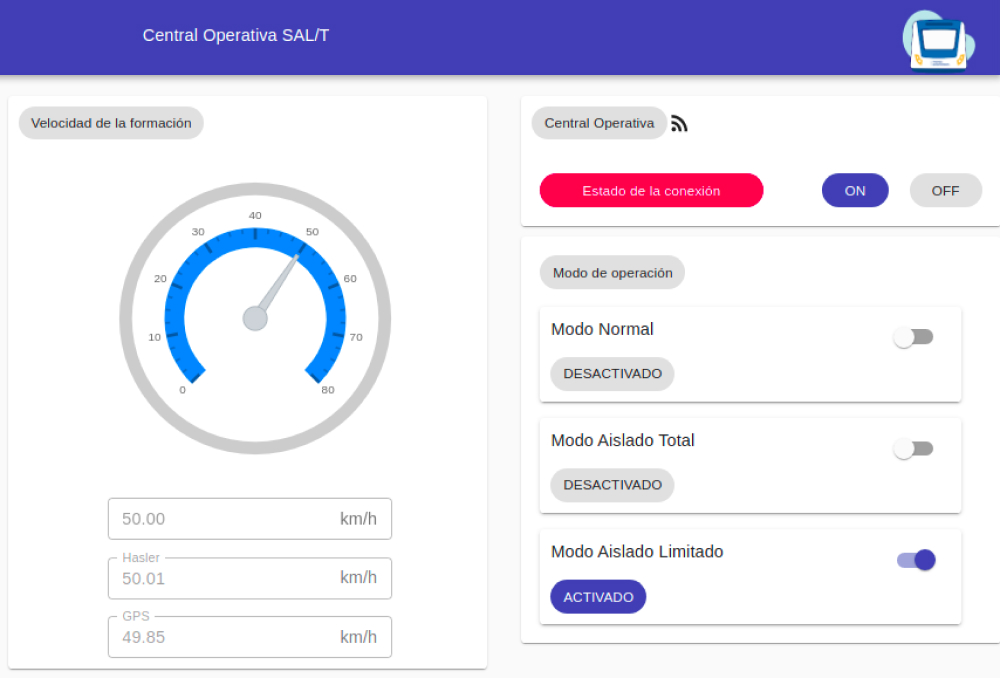
\includegraphics[width=.75\textwidth]{./Figures/dashboard.jpeg}
%	\caption{Panel de control de la Central Operativa SAL/T para la visualización de datos en tiempo real.}
%	\label{fig:dashboard}
%\end{figure}


\section{Motivación}

El sistema ferroviario de la República Argentina cuenta con una gran cantidad de formaciones ferroviarias en las que se encuentran diferentes sistemas de seguridad a bordo. Estos equipos se encargan de supervisar el correcto funcionamiento de los subsistemas críticos. Ante una falla en uno de los subsistemas, una formación ferroviaria se detiene inmediatamente por la activación automática de las señales de corte de tracción (\textit{CT}) y freno de emergencia (\textit{FE}). En esta situación, el conductor debe llevar la formación a un lugar seguro para que los pasajeros puedan descender y, posteriormente, trasladarla a un taller para que pueda ser reparada.

El \textit{SAL/T}, según sus siglas, Sistema de Aislamiento Limitado y Total \citep{salt-physical-paper}, es un dispositivo del cual se cuenta con una primera versión prototipada; que se presenta como solución a las contingencias descritas anteriormente. De esta manera, el maquinista de una formación ferroviaria cuenta con la posibilidad de activar y desactivar el \textit{modo aislado limitado}. En este modo, el equipo permite la circulación de la formación al desactivar las señales de corte de tracción y freno de emergencia generadas por los subsistemas críticos. Para que esta operación se complete de forma segura, se debe monitorear la velocidad de la formación tal que sea posible garantizar que no se supere cierto valor máximo.

A partir del desarrollo previo del prototipo, se presentan los avances en la implementación de una central operativa que centraliza los dispositivos \textit{SAL/T} para su respectiva administración, configuración y monitoreo en tiempo real de la información recibida y transmitida desde una plataforma digital. El trabajo se desarrolla por \textit{CONICET-GICSAFe} \citep{gicsafe} para la empresa Trenes Argentinos \citep{trenes-argentinos}.

Los subsistemas asociados al \textit{SAL/T}, como la seguridad de puertas, el sistema de hombre vivo y la protección de coche a la deriva, son críticos debido a que, en caso de fallar, pueden ocasionar lesiones o muertes de personas e incluso generar pérdidas materiales. 

La central operativa permite la administración y configuración en forma remota de los dispositivos de supervisión de seguridad de cada formación ferroviaria, la visualización de los diferentes parámetros de interés involucrados por las personas asignadas dentro de una entidad y de este modo es posible optimizar la toma de decisiones. 


\newpage
\section{Estado del arte}

A partir del análisis en las últimas tendencias referidas a la Central Operativa \textit{SAL/T}, se listan aquellas herramientas, de gestión y control de dispositivos de seguridad en el sector ferroviario, que presentan características similares al producto propuesto,

\begin{enumerate}

  \item \textit{Indra}\footnote{url{https://www.indracompany.com}}: ofrece una solución integral de seguridad para el sector ferroviario, que incluye una plataforma de gestión centralizada y un sistema de supervisión remota de dispositivos de seguridad.

  \item \textit{Thales Group}\footnote{url{https://www.thalesgroup.com}}: desarrolla soluciones de seguridad para el sector ferroviario, que incluyen una aplicación de gestión y control centralizada para supervisar y configurar dispositivos de seguridad de forma remota.

  \item \textit{Alstom}\footnote{url{https://www.alstom.com/}}: ofrece una plataforma de gestión y control para el sector ferroviario, que permite la supervisión y configuración de dispositivos de seguridad de forma remota, así como el análisis en tiempo real de los datos recopilados por estos dispositivos.

  \item \text{Siemens Mobility}\footnote{url{https://www.mobility.siemens.com/}}: ofrece una solución de gestión y control para el sector ferroviario, que incluye una aplicación web de central operativa para supervisar y configurar dispositivos de seguridad de forma remota, así como un sistema de análisis de datos en tiempo real.

\end{enumerate}


\section{Alcance y objetivos}

El sistema resultante de este trabajo se encuentra destinado al desarrollo del software para una central operativa que permite administrar y configurar de forma remota dispositivos de supervisión de seguridad de formaciones ferroviarias denominados \textit{SAL/T} (Sistema de Aislamiento Limitado/Total). 


El alcance del proyecto comprende los siguientes puntos,

\begin{itemize}
	\item Servicio de monitoreo y control: visualizar en tiempo real los datos recibidos y enviar comandos de control a los dispositivos activos. 

    \item Gestión de configuración de dispositivos: visualizar y modificar los parámetros configurables de los dispositivos. 

    \item Base de datos: registrar la información recibida desde todos los dispositivos.

    \item Componentes de seguridad: brindar seguridad a las comunicaciones y a la información almacenada. 

    \item Gestión de usuarios y perfiles: administrar roles y permisos de acceso.

    \item Realizar la migración de un microcontrolador de la familia Cortex tipo M \footnote{\url{https://developer.arm.com/Processors/Cortex-M4}} a uno de la misa familia que disponga de características destinadas a la seguridad funcional del sistema. 
\end{itemize}


\chapter{Introducción específica} % Main chapter title

\label{Chapter2}


%----------------------------------------------------------------------------------------
\section{Protocolos de comununicación utilizados}

  Comenzar escribiendo que aqui se detallaran los protocolos utilizados segun el modelo TCP/IP y hablar sobre el diagrama    

  AGREGAR UNA IMAGEN CON LOS 3 ENTES INTERCONECTADOS BAJO EL MODELO OSI 
        Nucleo F429ZI Board <----> Dedicated Server <----> Web Client


\subsection{Protocolos de comunicación}

De los modelos \textit{stack IoT} y \textit{lwIP} \citep{lwip}, basados en el stack \textit{TCP/IP} \footnote{\url{https://www.ibm.com/docs/en/aix/7.2?topic=protocol-tcpip-protocols}}, se emplean los siguientes protocolos de comunicación tal como se puede observar en la tabla \ref{tab:capa_protocolo}. 


\begin{table}[h]
\centering
\caption{Protocolos de comunicación utilizados en cada capa del \textit{stack TCP/IP}}
\label{tab:capa_protocolo}
\begin{tabular}{|c|c|}
\hline
\textbf{Capa} & \textbf{Protocolo} \\ \cline{1-2}
Capa de Aplicación & HTTP \citep{http}, DHCP \citep{dhcp} y MQTT \citep{mqtt} \\ \cline{1-2}
Capa de Transporte & UDP \citep{udp} \\ \cline{1-2}
Capa de Red & IPv4 \citep{ipv4}, ARP \citep{arp} \\ \cline{1-2}
Capa de Enlace de Datos & Ethernet \citep{ethernet} \\ \cline{1-2}
\end{tabular}
\end{table}

Cabe destacar que ambos modelos se encuentran diseñados para sistemas con recursos limitados y buscan garantizar una correcta comunicación entre los dispositivos conectados en la red.


%----------------------------------------------------------------------------------------
\section{Tecnologías \textit{full-stack}}

A partir de los modelos más relevantes que se encuentran establecidos para el desarrollo e implementación de aplicaciones de software se consideran el \textit{stack web} y el \textit{stack IoT}, tal como se puede ver en la figura \ref{fig:diagBloques}. A pesar de las similitudes entre ambos, en la aplicación el \textit{stack web} emplea el protocolo \textit{HTTP} mientras que el \textit{stack IoT} utiliza el protocolo \textit{MQTT}; siendo este último el más adecuado para escenarios donde son limitados los recursos como el ancho de banda y el consumo de energía.

En especial, el protocolo \textit{MQTT} dispone de mensajes más livianos y además es posible transmitir y/o recibir datos en formato binario sin la necesidad de una codificación previa. También, este protocolo permite asignar niveles de calidad de servicio (\textit{QoS} \footnote{\url{https://www.ibm.com/docs/en/i/7.2?topic=services-quality-service}}) a los mensajes transmitidos, resultando una característica primordial en aplicaciones donde la probabilidad de pérdidas de paquetes es considerable.


\begin{figure}[htpb]
  \centering 
  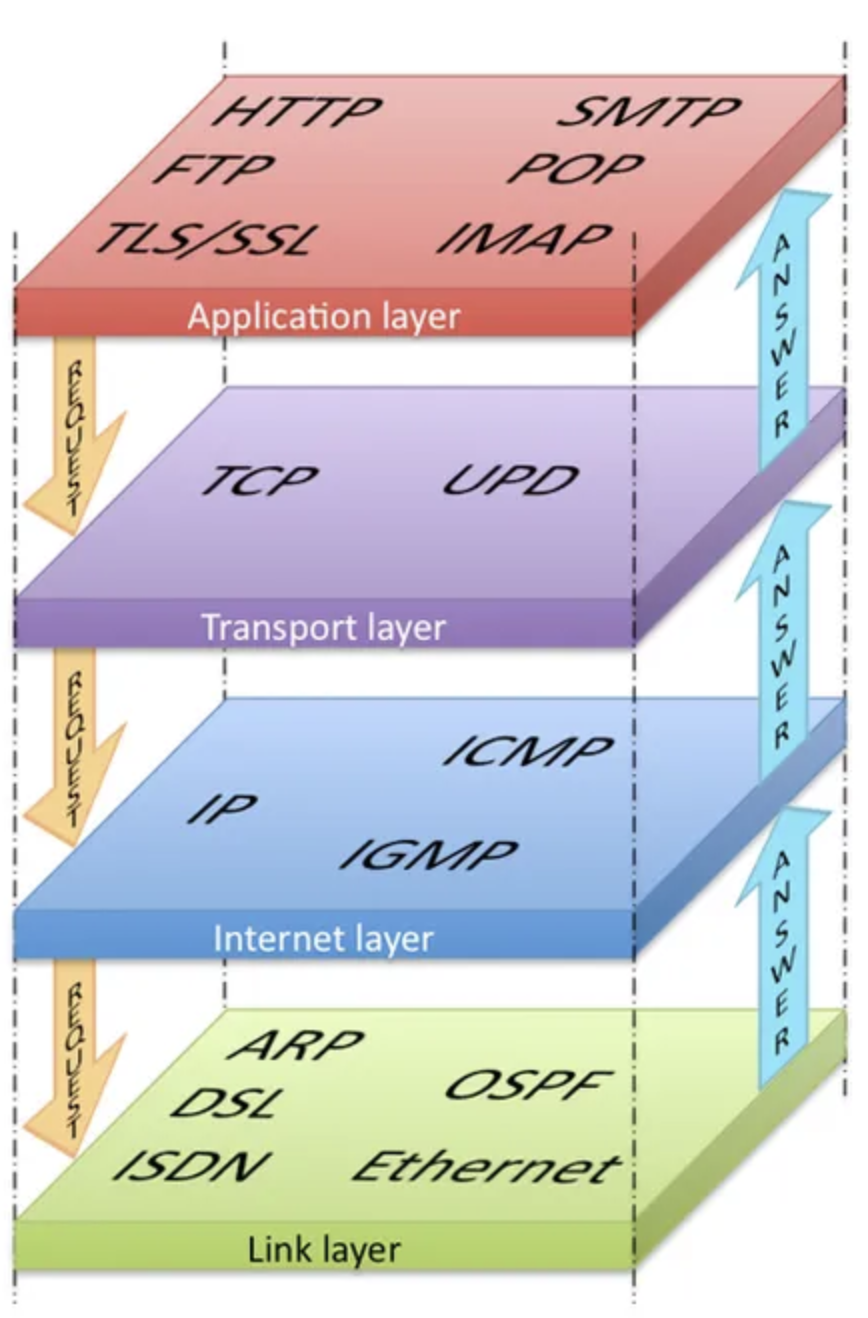
\includegraphics[width=.4\textwidth]{Figures/tcp-ip-stack.png}
  \caption{Arquitectura de la Central Operativa SAL/T.}
  \label{fig:diagBloques}
\end{figure}


\subsection{Tecnologías del \textit{front-end}}

\subsubsection{TypeScript}

TypeScript \citep{typescript} es una extensión de código abierto de JavaScript que agrega tipos estáticos opcionales y características de programación orientada a objetos avanzadas, lo que permite una mayor seguridad y mantenibilidad en el código. 


\subsubsection{React}

React \citep{react} es una biblioteca de JavaScript para construir UI reutilizables e interactivas, desarrollada por Facebook y ampliamente utilizada en el desarrollo web. Utiliza un enfoque basado en componentes y el DOM virtual para mejorar el rendimiento y es altamente integrable con otras bibliotecas y frameworks.


\subsubsection{Parcel}

Parcel \citep{parcel} es una herramienta de construcción de código abierto con una estrategia de "cero configuración" que optimiza y empaqueta módulos de JavaScript y otros archivos. En particular, mejora significativamente el flujo de trabajo del desarrollador al ser rápido, fácil de usar y altamente personalizable.


\subsubsection{Apollo GraphQL}

Apollo GraphQL \citep{apollo-graphql} es una plataforma de código abierto para el desarrollo de aplicaciones GraphQL, con una amplia gama de herramientas y servicios para construir y mantener aplicaciones GraphQL de manera efectiva, ofreciendo una administración de caché y una amplia compatibilidad con diferentes frameworks y tecnologías.


\subsubsection{Material UI}

Material UI \citep{material-ui} es una biblioteca de componentes de interfaz de usuario de código abierto basada en Material Design de Google, que ofrece componentes preconstruidos altamente personalizados y una amplia compatibilidad con diferentes tecnologías y frameworks para construir aplicaciones web modernas y atractivas.


\subsubsection{JWT Decode}

JWT Decode \citep{jwt-decode} es una biblioteca JavaScript que decodifica tokens JWT, con características útiles como validación de tokens y verificación de firma. Se integra fácilmente en diferentes frameworks de JavaScript como React y Angular.


%----------------------------------------------------------------------------------------
\subsection{Tecnologías del \textit{backend}}


\subsubsection{Kotlin}

Kotlin \citep{kotlin} es un lenguaje de programación de tipado estático que puede correr sobre la máquina virtual de Java y ser compilado en JavaScript y LLVM. También ofrece interoperabilidad con Java, programación funcional, orientación a objetos y manejo de nulos seguro, lo que ha llevado a su popularidad debido a su facilidad de uso y legibilidad.


\subsubsection{Ktor}

Ktor \citep{ktor} es un framework web de Kotlin que permite crear aplicaciones web y API REST de manera fácil y eficiente, con un enfoque en la programación funcional. Ktor es altamente modular y personalizable, lo que significa que los desarrolladores pueden seleccionar solo los componentes que necesitan para su aplicación, reduciendo así la complejidad y el tamaño del código. 


\subsubsection{Kafka}

Kafka \citep{kafka} es una plataforma de streaming de datos que permite a las aplicaciones enviar y recibir datos en tiempo real. Basada en el modelo de publicación/suscripción, se caracteriza por su alta velocidad y rendimiento, haciéndola ideal para aplicaciones que necesitan procesar grandes cantidades de datos en tiempo real.


\subsubsection{Hasura}

Hasura \citep{hasura} es una plataforma sin servidor que permite a los desarrolladores crear y escalar aplicaciones con GraphQL rápidamente. Ofrece seguridad de extremo a extremo y se integra fácilmente con diferentes bases de datos, generando automáticamente una API de GraphQL.


\subsubsection{PostgreSQL}

PostgreSQL \citep{postgresql} es un sistema de gestión de bases de datos de código abierto y gratuito, conocido por su fiabilidad, escalabilidad y seguridad. Ofrece soporte para transacciones ACID, integración con lenguajes de programación populares y una amplia variedad de herramientas y extensiones.


\subsubsection{Mosquitto Broker}

Mosquitto \citep{mosquitto} es un broker MQTT de código abierto utilizado en IoT para transmitir mensajes entre dispositivos. Es popular por su escalabilidad, facilidad de uso y características de seguridad.


%----------------------------------------------------------------------------------------
\subsection{Tecnologías del \textit{firmware}}


\subsubsection{C lang}

C \citep{c-lang} es un lenguaje de programación estructurado y de propósito general, ampliamente utilizado en sistemas operativos, aplicaciones de bajo nivel y dispositivos embebidos. Su sintaxis simple y directa permite escribir código claro y legible, y ofrece gran control sobre la memoria y acceso directo al hardware.


\subsubsection{FreeRTOS}

FreeRTOS \citep{free-rtos} es un RTOS de código abierto y gratuito que controla sistemas embebidos y microcontroladores, utilizado en control industrial, automoción y electrónica de consumo, con capacidad de rendimiento confiable y predecible. Es altamente portátil y ofrece gestión de tareas, semáforos, colas y temporizadores para sistemas complejos y eficientes en recursos.


\subsubsection{Paho MQTT \textit{client}}

Paho \citep{paho-mqtt} es una biblioteca cliente MQTT de código abierto que se utiliza para conectar aplicaciones a un broker MQTT. Paho es compatible con una amplia variedad de plataformas y lenguajes de programación, y ofrece una API sencilla para publicar y suscribir mensajes. Es ampliamente utilizado en aplicaciones de IoT y M2M para la transmisión eficiente de datos.


%----------------------------------------------------------------------------------------
\section{Herramientas utilizadas}


\subsubsection{Docker}

Docker \citep{docker} es una plataforma de software que permite a los desarrolladores crear, desplegar y ejecutar aplicaciones en contenedores. Estos contenedores permiten que las aplicaciones se ejecuten de manera aislada del sistema operativo y otras aplicaciones, lo que facilita su portabilidad y escalabilidad. 


\subsubsection{Docker Compose}

Docker Compose \citep{docker-compose} es una herramienta que permite definir y ejecutar aplicaciones de múltiples contenedores Docker. Permite a los desarrolladores especificar los servicios y la configuración de cada contenedor en un archivo YAML para simplificar la creación, ejecución y gestión de aplicaciones complejas. 


\subsubsection{Redpanda}

Redpanda \citep{redpanda} es una plataforma de streaming de datos distribuida y de alto rendimiento que combina las funcionalidades de Kafka y Redis. Es una solución escalable y confiable para el procesamiento de datos en tiempo real en entornos empresariales, y es compatible con una amplia variedad de casos de uso, desde el análisis de datos hasta la inteligencia artificial y el aprendizaje automático.


\subsubsection{Git}

Git \citep{git} es un sistema de control de versiones distribuido que se utiliza para rastrear los cambios en el código fuente de un proyecto de software. Permite a los desarrolladores trabajar en colaboración en el mismo código fuente y hacer un seguimiento de las diferentes versiones y ramas del proyecto. 


\subsubsection{MQTT.fx}

MQTT.fx \citep{mqtt-fx} es una herramienta de escritorio de código abierto que se utiliza para probar y depurar conexiones MQTT. Ofrece una interfaz gráfica de usuario fácil de usar para interactuar con brokers MQTT y suscribirse a temas y mensajes. MQTT.fx es compatible con una variedad de características de seguridad, como TLS/SSL y autenticación, lo que lo hace adecuado para su uso en entornos de producción.


\subsubsection{CLion}

CLion \citep{clion} es un entorno de desarrollo integrado (IDE) para programar en C y C++, que ofrece herramientas para la edición de código, depuración, refactorización y gestión de proyectos. Es conocido por su alta capacidad de análisis estático de código, lo que permite a los desarrolladores encontrar errores de forma eficiente.


\subsubsection{Wireshark}

Wireshark \citep{wireshark} es una herramienta de análisis de redes de código abierto y gratuita, utilizada para capturar y analizar paquetes de datos en tiempo real. Permite examinar el tráfico de red para identificar problemas de rendimiento, seguridad y configuración, y es compatible con una amplia variedad de protocolos de red.


\subsubsection{Herramientas del navegador de internet}

Las herramientas del navegador de Internet son características incorporadas en los navegadores web que permiten a los usuarios analizar y modificar elementos de una página web, como su estructura HTML, CSS y JavaScript. Algunas herramientas comunes incluyen la consola de desarrollador, el inspector de elementos, el depurador de JavaScript y el analizador de red, que ayudan a los desarrolladores a depurar problemas y mejorar la calidad de sus sitios web.


\subsubsection{JTAG}

JTAG (Joint Test Action Group) \citep{jtag} es un estándar para la depuración y programación de dispositivos electrónicos. Permite acceder a los pines de prueba de un dispositivo para realizar pruebas de hardware y depuración a nivel de circuito. JTAG se ha convertido en un estándar común para la depuración y programación de dispositivos, y muchas herramientas de desarrollo de software y hardware lo admiten.


\subsubsection{ST-Link}

ST-Link \citep{st-link} es una herramienta de programación y depuración de microcontroladores fabricada por STMicroelectronics. Se utiliza para programar y depurar microcontroladores STM32 y otros dispositivos compatibles con JTAG o SWD. La herramienta se conecta al ordenador mediante USB y se puede usar con una variedad de entornos de desarrollo integrados (IDE) y herramientas de depuración. 


\subsubsection{STM32CubeMX}

STM32CubeMX \citep{stm32-cubemx} es una herramienta de configuración gráfica para dispositivos STM32 que permite a los desarrolladores generar automáticamente código inicial para su proyecto. Ofrece una interfaz de usuario intuitiva que simplifica la configuración de periféricos y pines, y admite una variedad de opciones de generación de código. 


\subsubsection{STM32CubeProgrammer}

STM32CubeProgrammer \citep{stm32-cubeprogrammer} es una herramienta de programación y actualización de firmware para dispositivos STM32 que permite programar y depurar dispositivos STM32, así como actualizar su firmware en campo. Es compatible con una variedad de interfaces de programación, como JTAG, SWD y UART, y es fácil de usar gracias a su interfaz gráfica de usuario. 



 
\chapter{Diseño e implementación} % Main chapter title

\label{Chapter3} % Change X to a consecutive number; for referencing this chapter elsewhere, use \ref{ChapterX}


\section{Descripción del sistema}


\textbf{PARAFRASEAR EL PRIMER PARRAFO PORQUE SE REPITE CON LA MOTIVACION DEL PROYECTO !}

El \textit{SAL/T}, según sus siglas, Sistema de Aislamiento Limitado o Total, es un sistema que le permitirá al conductor la activación y desactivación del modo aislado limitado. En este modo, el equipo permite la circulación de la formación al desactivar las señales de corte de tracción y freno de emergencia generadas por los otros subsistemas. Para que esta operación se realice de forma segura, se debe monitorear la velocidad de la formación tal que sea posible evitar que supere cierto valor máximo. 
Se considera un sistema crítico debido a que, en caso de fallar, puede ocasionar lesiones o muertes de personas, dañar el medio ambiente y/o generar grandes pérdidas materiales.

En trabajos anteriores se desarrollaron las primeras cinco fases de catorce que componen el ciclo de vida según la norma \textit{UNE-EN 50126}, centradas en el relevamiento de la necesidad y la obtención de los requerimientos técnicos del sistema.

En la actualidad, existe un prototipo de este sistema que fue finalizado en el año 2019, del cual, en lo que respecta al \textit{firmware}, se propone realizar la migración a un microcontrolador de la familia \textit{Cortex} tipo M con mayor soporte al actual y que cuente con funcionalidades de seguridad.  

Por otro lado, tal como se puede observar en el margen inferior derecho de la figura 1, se plantea el desarrollo de una central operativa. Se trata de una plataforma web que cuenta con una unidad lógica de compartición y empaquetado de software posibilitando la administación, la configuración y el monitoreo en tiempo real de la información recibida y transmitida por parte de cada dispositivo SAL/T. 


\newpage
En caso de ser necesario, a partir de la activación de una señal crítica provista por el artefacto \textit{Hasler} \footnote{ es un sistema electromecánico que registra los eventos de velocidad del material rodante, la señal de anuncio y la señal de frenado automático.
}  que se encuentra instalado en cada formación ferroviaria, un operario puede accionar alguno de los comandos que se listan a continuación:


\begin{itemize}
	\item \textbf{Modo aislado total}: se habilita la tracción y se libera el freno de emergencia, independientemente de cualquier condición. 

    \item \textbf{Modo coche en deriva}: se corta la tracción y se libera el freno de emergencia, independientemente de cualquier condición. 

    \item \textbf{Modo parada total}: se corta la tracción y se aplica el freno de emergencia, independientemente de cualquier condición. 
    
    \item \textbf{Modo intermitente}: se habilita la tracción y se aplica el freno de emergencia en ciclos de tiempo configurables. 

    \item Anulación de comandos remotos vigentes.

\end{itemize}


Para el seguimiento de las variables, publicadas por cada dispositivo SAL/T, que permiten la visualización en la plataforma, se realiza la suscripción a un tópico del \textit{broker} \textit{MQTT} y se registra la información indexada en la base de datos de un servidor. En consecuencia, resulta de extrema importancia que la comunicación a través de \textit{MQTT} opere sobre el protocolo de encriptación \textit{SSL/TSL}, de modo que se exponga un considerable nivel de seguridad; de igual manera, es necesaria la utilización de certificados para el acceso a la lectura y la escritura en la base de datos.  

Así mismo, es necesario que la página web ofrezca la configuración de los parámetros de cada dispositivo conectado a la formación ferroviaria, la administración de los roles y la autenticación de los usuarios.

\begin{figure}[htpb]
\centering 
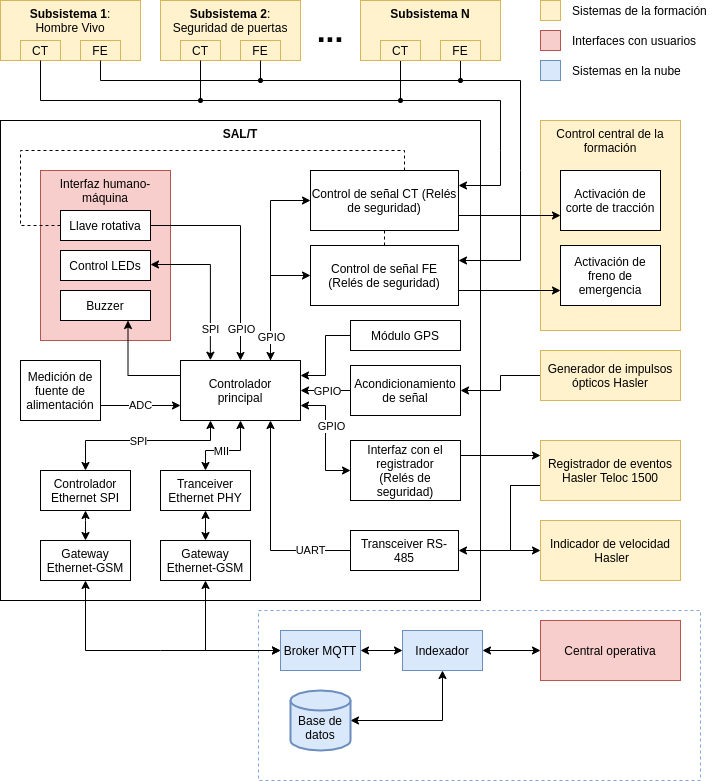
\includegraphics[width=.8\textwidth]{Figures/diagrama_salt_con_central.png}
\caption{Diagrama en bloques del sistema SALT.}
\label{fig:diagBloques}
\end{figure}

\subsection{Comunicación device y backend}

MQTT

Ver cuanto se repite con el ultimo parrafo de arriba.

\subsection{Comunicación backend y frontend}

HTTP

Ver cuanto se repite con el ultimo parrafo de arriba.


\section{Arquitectura del sistema}


\textbf{PARAFRASEAR EL PRIMER PARRAFO PORQUE SE REPITE CON LA MOTIVACION DEL PROYECTO !}

A partir de los modelos más relevantes que se encuentran establecidos para el desarrollo e implementación de aplicaciones de software se consideran el \textit{stack web} y el \textit{stack IoT}. A pesar de las similitudes entre ambos, en la aplicación el \textit{stack web} emplea el protocolo \textit{HTTP} mientras que el \textit{stack IoT} utiliza el protocolo \textit{MQTT}; siendo este último el más adecuado para escenarios donde son limitados los recursos como el ancho de banda y el consumo de energía.

En especial, el protocolo \textit{MQTT} dispone de mensajes más livianos y además es posible transmitir y/o recibir datos en formato binario sin la necesidad de una codificación previa. También, este protocolo permite asignar niveles de calidad de servicio (\textit{QoS}) a los mensajes transmitidos, resultando una característica primordial en aplicaciones donde la probabilidad de pérdidas de paquetes es considerable.

La \textbf{figura X} presenta la estratificación de las capas, según el \textit{stack IoT}, que son detalladas a lo largo de esta sección.


\textbf{AGREGAR NUEVA FIGURA SUPER GENERAL DEL STACK IOT CON SUS CAPAS}


\subsection{Capa de dispositivos}

Sobre la base de un prototipo del Sistema de Aislamiento Limitado o Total, \textit{SAL/T}, se desarrolló mediante el kit de desarrollo \textit{Nucleo F429} \citep{nucleo-kit}, un cliente \textit{MQTT} que permite la publicación de la velocidad de la formación y de los parámetros provistos por los subsistemas de falla, entre otras variables; y llegado el caso, el dispositivo pueda realizar la lectura de diferentes parámetros configurables.

\subsection{Capa de conectividad}

Para la comunicación entre los dispositivos \textit{SAL/T} y la capa de almacenamiento se emplea un \textit{Broker MQTT} que oficia de orquestador entre el cliente, el dispositivo \textit{SAL/T} que publica los mensajes y \textit{Apache Kafka}, un sistema distribuido que efectúa la lectura de la información y su posterior procesamiento. 

Dado que los mensajes intercambiados entre las partes contienen información sensible, se ha optado por agregar la capa de seguridad \textit{TLS}. En este sentido, resulta indispensable utilizar el certificado \textit{X509} para prevenir ataques del tipo \textit{adversary-in-the-middle} y los certificados emitidos por autoridades reconocidas.


\subsection{Capa de almacenamiento}

La capa de almacenamiento se encuentra constituida por el sistema distribuido \textit{Kafka} que se encarga de almacenar los datos de la aplicación. Entre ellos se destacan los mensajes MQTT enviados por los dispositivos SAL/T, como también la información referida a las formaciones y a los SAL/T que las ocupan. Además, se tienen servicios de procesamiento de datos que se encargan de adaptar la información de los tópicos en datos que posteriormente serán consumidos por los servicios que integran la capa superior.

Por otro lado, se tiene una base de datos relacional \textit{PostgreSQL} para el almacenamiento de los datos provenientes del servicio de autenticación y el motor que facilita la interacción con la plataforma web. Los conectores se encargan de insertar los datos que se quieran disponer a la capa de visualización.


En la figura \textbf{devicesTrainEntity} se observa el modelo de datos que representa a los dispositivos SAL/T, las formaciones y las entidades. 
El primero cuenta con un identificador del dispositivo en el sistema, el estado de operación y una referencia al tren en el que se desplegó el artefacto. 
El modelo de la formación está enriquecido con la entidad a la que pertenece y el número de serie del tren. 
Por último, las entidades están compuestas por nombre y descripción.
En la figura \textbf{devicesSubsystems} se aprecian los subsistemas de fallas relacionados con el dispositivo SAL/T. Su modelo está integrado con el nombre del subsistema, el identificador del dispositivo al que está asociado y el estado actual del mismo. 

\subsection{Capa de interacción}

La capa de interacción se encuentra conformada por tres unidades. Por un lado, se ha desarrollado en el lenguaje \textit{Kotlin} en conjunto con el \textit{framework} \textit{Ktor}, un microservicio de autenticación donde es posible la gestión de los usuarios con sus respectivos roles y también el \textit{backend}. Entre sus tareas principales se encuentran las relacionadas con el protocolo \textit{MQTT} para la actualización de los certificados que brindan seguridad a las comunicaciones, mediante el uso de la capa de seguridad \textit{TLS}, y la indexación de los eventos que se publiquen en tiempo real; como la configuración general que permite el funcionamiento integral de los servicios y módulos dispuestos en el sistema. \\

Además, se dispone del motor \textit{Hasura}, el cual se encuentra conectado a una base de datos relacional (\textit{PostgreSQL}) basado en el lenguaje de consulta estructurado \textit{SQL}, que permite exponer una \textit{API GraphQL} a aquellos clientes que deseen obtener una visualización del modelo de datos propuesto en que se conjuga la información de cada formación ferroviaria con su correspondiente dispositivo \textit{SAL/T} y diseño destinado al \textit{frontend}. Más aún, el enlace permite realizar modificaciones y hasta remociones de las columnas propuestas en las tablas de cada esquema dentro de la base de datos.


\subsection{Capa de visualización}

En esta capa se ha utilizado el lenguaje de programación \textit{TypeScript} junto con la biblioteca gráfica \textit{React} para brindar una web reactiva en la que se elaboraron los formularios, las tablas y los paneles a partir de la explotación de la información almacenada en la base de datos. Cabe destacar que la plataforma web se encuentra condicionada por el rol y la entidad a la que pertenece cada usuario, de modo que, cada formación ferroviaria tendrá un operador asignado, el cual podrá modificar los parámetros correspondientes con el dispositivo asociado.

En la figura \textbf{dashboard} se puede apreciar el panel de control de la central operativa al que tendrán acceso los operadores de cada entidad.
En el mismo se observan distintas tarjetas con el estado de cada subsistema de fallas y del tren, como así también un velocímetro que informa la velocidad de la formación.

\newpage
\section{Arquitectura de datos}

Para crear la estructura de la base de datos SQL, se realiza un análisis detallado del sistema y se identifican las principales entidades: la formación ferroviaria, los subsistemas de falla y las áreas. Toda la información de estas entidades se nuclea en la entidad tren, la cual representa una formación ferroviaria con todos sus subsistemas y áreas asociadas. A partir del modelado de estas entidades y sus atributos correspondientes, se definen las relaciones entre ellas y se establecen las claves primarias y foráneas.


Para visualizar de manera más clara la estructura de la base de datos y sus relaciones, se utiliza el diagrama UML (Lenguaje de Modelado Unificado). En la siguiente figura se muestra el diagrama UML de la base de datos, donde se pueden observar las diferentes entidades, sus atributos y relaciones. A partir de este diagrama se procede a crear las tablas en la base de datos SQL y a definir sus columnas y restricciones, garantizando así la integridad de los datos y el correcto funcionamiento del sistema.


\textbf{CONTINUAR CON EL DIAGRAMA UML CONECTANDO LAS ENTIDADES  \\ VER Figures/salt\_uml\_drawio}
\url{https://app.diagrams.net/}


\subsection{Entidades del modelo de datos}


\textbf{COMENTAR SI ES QUE LAS HAY, PARTICULARIDADES SOBRE CADA UNA DE LAS ETIDADES DEL SISTEMA Y CADA TABLA DEL DIAGRAMA UML}

 
\subsubsection{Schema auth\_service}

\begin{itemize}

\item \textbf{credentials}: Esta tabla almacena las credenciales de los usuarios para acceder al sistema. Tiene una clave foránea a la tabla \textbf{auth\_service users} y es referenciada por la tabla \textbf{auth\_service roles}.

\item \textbf{roles}: Esta tabla almacena los roles de los usuarios. Tiene una clave foránea a la tabla \textbf{auth\_service users} y es referenciada por la tabla \textbf{enums roles}.

\item \textbf{users}: Esta tabla almacena la información básica de los usuarios del sistema. Es referenciada por la tabla \textbf{auth\_service credentials} y la tabla \textbf{public users}.

\end{itemize}


\subsubsection{Schema enums}

\begin{itemize}

  \item \textbf{device status}: Esta tabla almacena los estados posibles para los dispositivos. Es referenciada por la tabla \textbf{public devices}.

  \item \textbf{events}: Esta tabla almacena los tipos de eventos posibles. Es referenciada por la tabla \textbf{public internal events}.

  \item \textbf{fail system}: Esta tabla almacena los sistemas de falla posibles. Es referenciada por la tabla \textbf{public remote events} y la tabla \textbf{public subsystems}.

  \item \textbf{roles}: Esta tabla almacena los roles posibles para los usuarios del sistema. Es referenciada por la tabla \textbf{auth\_service roles}.

\end{itemize}


\subsubsection{Schema public}

\begin{itemize}

\item \textbf{devices}: Esta tabla almacena información sobre los dispositivos del sistema. Tiene una clave foránea a la tabla \textbf{public train} y es referenciada por la tabla \textbf{public remote events} y la tabla \textbf{public internal events}.

\item \textbf{entities}: Esta tabla almacena información sobre las entidades del sistema. Es referenciada por la tabla \textbf{public train}.

\item \textbf{internal events}: Esta tabla almacena información sobre los eventos internos del sistema. Tiene claves foráneas a las tablas \textbf{public devices}, \textbf{enums events} y \textbf{public users}.

\item \textbf{remote events}: Esta tabla almacena información sobre los eventos remotos del sistema. Tiene una clave foránea a la tabla \textbf{public devices} y es referenciada por la tabla \textbf{enums fail system}.

\item \textbf{subsystems}: Esta tabla almacena información sobre los subsistemas del sistema. Tiene una clave foránea a la tabla \textbf{public devices} y es referenciada por la tabla \textbf{enums fail system}.

\item \textbf{train}: Esta tabla almacena información sobre los trenes del sistema. Tiene una clave foránea a la tabla \textbf{public entities} y es referenciada por la tabla \textbf{public devices}.

\item \textbf{user data}: Esta tabla almacena información adicional de los usuarios del sistema. Es referenciada por la tabla \textbf{public users}.

\item \textbf{users}: tabla que contiene información de los usuarios. Tiene una relación de clave externa con la tabla entities.


\end{itemize}






\section{Seguridad del sistema}

\subsection{Protocolo HTTPS}

security layer

jwt

\textbf{Referencia - pag 44}
https://lse-posgrados-files.fi.uba.ar/tesis/LSE-FIUBA-Trabajo-Final-CEIoT-Pedro-Rosito-2021.pdf


\subsection{MQTT v5.0}

payload encryption



\section{Desarrollo del frontend}

\textbf{AGREGAR UNA BREVE INTRO SOBRE QUE SE EXPONDRA AQUI}
\textit{tipos de clientes, apollo client, codegen, }

\subsection{Estructura del cliente web}

\begin{enumerate}

  \item index html

  \item main tsx 

  \item react router -> pages

\end{enumerate}


\subsection{Páginas}

\textbf{HABLAR DE CADA PAGINA A PARTIR DE UNA IMAGEN DONDE SE MUESTRE EL SIDEBAR}

\textit{dashboard, sign in, configuration, entities, trains, subsystems of each train, logs, etc}

\subsubsection{Login}

\textbf{hablar sobre jwt}
\textit{Referecia - bastian pag 48}

\textbf{add figure}


\subsubsection{Tabla de trenes+salt}

\textbf{add figure}


\subsubsection{Tabla de usuarios}

\textbf{add figure}


\subsubsection{dashboard}

\textbf{add figure}

\subsection{Modales}

\textit{crear: usuario, tren, dispositivo ; configuracion: sub sistemas de seguridad, etc}





\section{Desarrollo del backend}


A partir del uso de archivo docker-compose, que se ejecuta en un entorno Docker, para proporcionar el conjunto completo de servicios para enviar, recibir y almacenar los datos a través de diferentes protocolos. Cada servicio se ejecuta en su propio contenedor y se conecta a los otros servicios según el siguiente formato:


\textbf{AGREGAR IMAGEN DEL ENTORNO DOCKER CON SUS CONTENEDORES Y CONEXIONES }
\url{https://www.gotoiot.com/pages/articles/docker_intro/index.html}
\url{https://www.gotoiot.com/pages/articles/docker_intro/images/image2.png}


\begin{itemize}

  \item mosquitto: es un servidor MQTT de código abierto que se utiliza para enviar y recibir mensajes. Se utiliza la imagen "eclipse-mosquitto" y se mapea el puerto 1883 en el host al puerto 1883 en el contenedor. También se montan dos volúmenes, uno para la configuración del servidor y otro para los datos.

  \item hasura: es un motor de GraphQL que proporciona una API para interactuar con una base de datos. Se utiliza la imagen "hasura/graphql-engine:v2.1.0" y se mapea el puerto 8080 en el host al puerto 8080 en el contenedor. Se configuran varias variables de entorno, incluyendo la URL de la base de datos y el secreto de administrador. También depende del servicio "postgres".

  \item postgres: es una base de datos relacional que se utiliza para almacenar datos. Se utiliza la imagen "postgres:13" y se mapea el puerto 5432 en el host al puerto 5432 en el contenedor. Se configuran varias variables de entorno, incluyendo el nombre de la base de datos, el nombre de usuario y la contraseña. También se monta un volumen para almacenar los datos de la base de datos.

  \item zookeeper: es un servicio que se utiliza para coordinar los nodos de Kafka. Se utiliza la imagen "confluentinc/cp-zookeeper:6.2.4" y se configura el puerto de cliente en 2181.

  \item kafka: es un servicio de mensajería de código abierto que se utiliza para enviar y recibir mensajes. Se utiliza la imagen "confluentinc/cp-kafka:6.2.4" y se mapea el puerto 9092 en el host al puerto 9092 en el contenedor. Se configuran varias variables de entorno, incluyendo la conexión de Zookeeper y el número de réplicas de las particiones. También depende del servicio "zookeeper".

  \item kafka-ui: es una interfaz de usuario para administrar y monitorear clústeres de Kafka. Se utiliza la imagen "provectuslabs/kafka-ui" y se mapea el puerto 8085 en el host al puerto 8080 en el contenedor. Se configuran varias variables de entorno, incluyendo la conexión al clúster de Kafka, el esquema de registro y el servidor de KSQLDB.

\end{itemize}


\subsubsection{Mosquitto Broker}

\textbf{TALK ABOUT THE MOSQUITTO CONFIG FILE AND THE CLI INSTALLATION, USAGE, ETC.}


\subsubsection{Hasura}

\textbf{TALK ABOUT HASURA GUI, CLI AND USAGE. ADD AN EXAMPLE QUERY}


\subsubsection{Kafka}

\textbf{TALK ABOUT KAFKA AND REDPANDA. ADD AN EXAMPLE QUERY}


\section{Desarrollo del firmware}

\textbf{Explicar como se combinan todas las tecnologias y herramientas en el firmware. basarlo en el stack lwip}

\textbf{Referecia - pagina 43}
\textit{https://lse-posgrados-files.fi.uba.ar/tesis/LSE-FIUBA-Trabajo-Final-CEIoT-Pedro-Rosito-2021.pdf }


\begin{itemize}

  \item based on: \url{https://blog.naver.com/eziya76/221938551688}

  \item nucleo F429ZI kit development

  \item free rtos

  \item tools: cube mx, cube programmer, mosquitto cli

\end{itemize}



\section{Desarrollo de la API GraphQL}

\textbf{Referencias}

\begin{itemize}

  %https://github.com/Azure-Samples/blockchain/blob/master/blockchain-workbench/rest-api-samples/java/generated/docs/ApplicationsApi.md#applicationDelete
  
  \item https://github.com/nandroidj/app-fullstack-base-2021-1c
    \\ \textit{Detalles de implementación -> Ver los endpoints disponibles}

  \item https://www.notion.so/briken/KoyweTransaction-8d9ba1eda4664819a30378c3548ebacf?pvs=4

  \item https://www.notion.so/briken/User-2ad1013d829548d0a7e992e31e53f7df?pvs=4

\end{itemize}



%% Chapter Template

\chapter{Ensayos y resultados} % Main chapter title

\label{Chapter4} % Change X to a consecutive number; for referencing this chapter elsewhere, use \ref{ChapterX}

%----------------------------------------------------------------------------------------
%	SECTION 1
%----------------------------------------------------------------------------------------

\section{Pruebas funcionales del hardware}
\label{sec:pruebasHW}

La idea de esta sección es explicar cómo se hicieron los ensayos, qué resultados se obtuvieron y analizarlos.
 
%% Chapter Template

\chapter{Conclusiones} % Main chapter title

\label{Chapter5} % Change X to a consecutive number; for referencing this chapter elsewhere, use \ref{ChapterX}


%----------------------------------------------------------------------------------------

%----------------------------------------------------------------------------------------
%	SECTION 1
%----------------------------------------------------------------------------------------

\section{Conclusiones generales }

La idea de esta sección es resaltar cuáles son los principales aportes del trabajo realizado y cómo se podría continuar. Debe ser especialmente breve y concisa. Es buena idea usar un listado para enumerar los logros obtenidos.

Algunas preguntas que pueden servir para completar este capítulo:

\begin{itemize}
\item ¿Cuál es el grado de cumplimiento de los requerimientos?
\item ¿Cuán fielmente se puedo seguir la planificación original (cronograma incluido)?
\item ¿Se manifestó algunos de los riesgos identificados en la planificación? ¿Fue efectivo el plan de mitigación? ¿Se debió aplicar alguna otra acción no contemplada previamente?
\item Si se debieron hacer modificaciones a lo planificado ¿Cuáles fueron las causas y los efectos?
\item ¿Qué técnicas resultaron útiles para el desarrollo del proyecto y cuáles no tanto?
\end{itemize}


%----------------------------------------------------------------------------------------
%	SECTION 2
%----------------------------------------------------------------------------------------
\section{Próximos pasos}

Acá se indica cómo se podría continuar el trabajo más adelante.
 

%----------------------------------------------------------------------------------------
%	CONTENIDO DE LA MEMORIA  - APÉNDICES
%----------------------------------------------------------------------------------------

\appendix % indicativo para indicarle a LaTeX los siguientes "capítulos" son apéndices

% Incluir los apéndices de la memoria como archivos separadas desde la carpeta Appendices
% Descomentar las líneas a medida que se escriben los apéndices

%% Appendix A

\chapter{Appendix Title Here} % Main appendix title

\label{AppendixA} % For referencing this appendix elsewhere, use \ref{AppendixA}

Write your Appendix content here.
%\include{Appendices/AppendixB}
%\include{Appendices/AppendixC}

%----------------------------------------------------------------------------------------
%	BIBLIOGRAPHY
%----------------------------------------------------------------------------------------

\Urlmuskip=0mu plus 1mu\relax
\raggedright
\printbibliography[heading=bibintoc]

%\begin{thebibliography}{00}
%
%\bibitem{b1} 'Sistema de supervisión de la seguridad del material
%ferroviario utilizando patrones de diseño', Ivan Mariano Di Vito, Pablo Gomez, Ariel Lutenberg, Libro de trabajos del CASE2019, Congreso Argetino de Sistemas Embebidos, Santa Fe, Argentina. (2019).
%
%\bibitem{b2} CONICET-GICSAFe (June 2022). [Online]. Disponible: \\ https://sites.google.com/view/conicet-gicsafe/inicio
%
%\bibitem{b3} Trenes Argentinos (June 2022). [Online]. Disponible: \\ https://www.argentina.gob.ar/transporte/trenes 
%
%\end{thebibliography}

%----------------------------------------------------------------------------------------

\end{document}  
